\documentclass{scrartcl}
        \usepackage{xcolor, tikz}
        \usepackage{pgfplots}
        \pgfplotsset{compat=newest}
        \pagestyle{empty}
        \definecolor{pdg2112}{RGB}{228,26,28}
\definecolor{pdg2212}{RGB}{55,126,184}
\definecolor{pdg1000020040}{RGB}{166,86,40}
\definecolor{pdg11}{RGB}{152,78,163}
\definecolor{pdg12}{RGB}{255,127,0}
\definecolor{pdg1000030060}{RGB}{153,153,153}
\definecolor{pdg1000030070}{RGB}{153,153,153}
\definecolor{pdg22}{RGB}{77,175,74}
\definecolor{pdg1000060120}{RGB}{153,153,153}
\definecolor{pdg1000040090}{RGB}{153,153,153}
\begin{document}
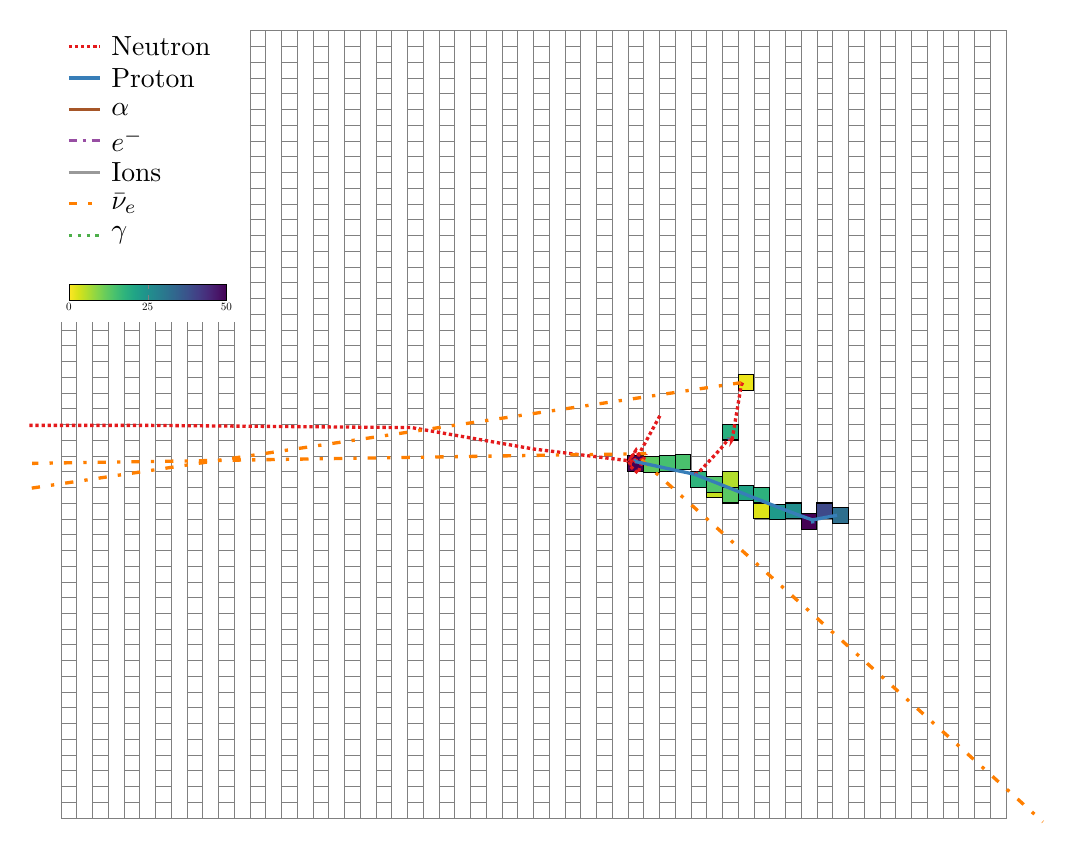
\begin{tikzpicture}[scale=0.4] %\columnwidth/252.0pt]
\draw[step=0.5,very thin,gray] (-0.001000,-12.499) grid (0.500000,3.25);
\draw[step=0.5,very thin,gray] (0.999000,-12.499) grid (1.500000,3.25);
\draw[step=0.5,very thin,gray] (1.999000,-12.499) grid (2.500000,3.25);
\draw[step=0.5,very thin,gray] (2.999000,-12.499) grid (3.500000,3.25);
\draw[step=0.5,very thin,gray] (3.999000,-12.499) grid (4.500000,3.25);
\draw[step=0.5,very thin,gray] (4.999000,-12.499) grid (5.500000,3.25);
\draw[step=0.5,very thin,gray] (5.999000,-12.499) grid (6.500000,12.499);
\draw[step=0.5,very thin,gray] (6.999000,-12.499) grid (7.500000,12.499);
\draw[step=0.5,very thin,gray] (7.999000,-12.499) grid (8.500000,12.499);
\draw[step=0.5,very thin,gray] (8.999000,-12.499) grid (9.500000,12.499);
\draw[step=0.5,very thin,gray] (9.999000,-12.499) grid (10.500000,12.499);
\draw[step=0.5,very thin,gray] (10.999000,-12.499) grid (11.500000,12.499);
\draw[step=0.5,very thin,gray] (11.999000,-12.499) grid (12.500000,12.499);
\draw[step=0.5,very thin,gray] (12.999000,-12.499) grid (13.500000,12.499);
\draw[step=0.5,very thin,gray] (13.999000,-12.499) grid (14.500000,12.499);
\draw[step=0.5,very thin,gray] (14.999000,-12.499) grid (15.500000,12.499);
\draw[step=0.5,very thin,gray] (15.999000,-12.499) grid (16.500000,12.499);
\draw[step=0.5,very thin,gray] (16.999000,-12.499) grid (17.500000,12.499);
\draw[step=0.5,very thin,gray] (17.999000,-12.499) grid (18.500000,12.499);
\draw[step=0.5,very thin,gray] (18.999000,-12.499) grid (19.500000,12.499);
\draw[step=0.5,very thin,gray] (19.999000,-12.499) grid (20.500000,12.499);
\draw[step=0.5,very thin,gray] (20.999000,-12.499) grid (21.500000,12.499);
\draw[step=0.5,very thin,gray] (21.999000,-12.499) grid (22.500000,12.499);
\draw[step=0.5,very thin,gray] (22.999000,-12.499) grid (23.500000,12.499);
\draw[step=0.5,very thin,gray] (23.999000,-12.499) grid (24.500000,12.499);
\draw[step=0.5,very thin,gray] (24.999000,-12.499) grid (25.500000,12.499);
\draw[step=0.5,very thin,gray] (25.999000,-12.499) grid (26.500000,12.499);
\draw[step=0.5,very thin,gray] (26.999000,-12.499) grid (27.500000,12.499);
\draw[step=0.5,very thin,gray] (27.999000,-12.499) grid (28.500000,12.499);
\draw[step=0.5,very thin,gray] (28.999000,-12.499) grid (29.500000,12.499);
\draw[very thin,gray] (0,-12.5) -- (30,-12.5) -- (30,12.5) -- (6,12.5);
\definecolor{tempcolor}{rgb}{0.267004,0.004874,0.329415}\draw[fill=tempcolor,fill opacity=1] (18.000000,-1.500000) rectangle (18.500000,-1.000000);
\definecolor{tempcolor}{rgb}{0.369214,0.788888,0.382914}\draw[fill=tempcolor,fill opacity=1] (18.500000,-1.520491) rectangle (19.000000,-1.020491);
\definecolor{tempcolor}{rgb}{0.274149,0.751988,0.436601}\draw[fill=tempcolor,fill opacity=1] (19.000000,-1.500000) rectangle (19.500000,-1.000000);
\definecolor{tempcolor}{rgb}{0.288921,0.758394,0.428426}\draw[fill=tempcolor,fill opacity=1] (19.500000,-1.448804) rectangle (20.000000,-0.948804);
\definecolor{tempcolor}{rgb}{0.185783,0.704891,0.485273}\draw[fill=tempcolor,fill opacity=1] (20.000000,-2.000000) rectangle (20.500000,-1.500000);
\definecolor{tempcolor}{rgb}{0.772852,0.877868,0.131109}\draw[fill=tempcolor,fill opacity=1] (20.500000,-2.330646) rectangle (21.000000,-1.830646);
\definecolor{tempcolor}{rgb}{0.311925,0.767822,0.415586}\draw[fill=tempcolor,fill opacity=1] (20.500000,-2.155353) rectangle (21.000000,-1.655353);
\definecolor{tempcolor}{rgb}{0.352360,0.783011,0.392636}\draw[fill=tempcolor,fill opacity=1] (21.000000,-2.500000) rectangle (21.500000,-2.000000);
\definecolor{tempcolor}{rgb}{0.699415,0.867117,0.175971}\draw[fill=tempcolor,fill opacity=1] (21.000000,-2.000000) rectangle (21.500000,-1.500000);
\definecolor{tempcolor}{rgb}{0.162016,0.687316,0.499129}\draw[fill=tempcolor,fill opacity=1] (21.000000,-0.500000) rectangle (21.500000,0.000000);
\definecolor{tempcolor}{rgb}{0.926106,0.897330,0.104071}\draw[fill=tempcolor,fill opacity=1] (21.500000,1.078380) rectangle (22.000000,1.578380);
\definecolor{tempcolor}{rgb}{0.124780,0.640461,0.527068}\draw[fill=tempcolor,fill opacity=1] (21.500000,-2.429876) rectangle (22.000000,-1.929876);
\definecolor{tempcolor}{rgb}{0.876168,0.891125,0.095250}\draw[fill=tempcolor,fill opacity=1] (22.000000,-3.000000) rectangle (22.500000,-2.500000);
\definecolor{tempcolor}{rgb}{0.175707,0.697900,0.491033}\draw[fill=tempcolor,fill opacity=1] (22.000000,-2.500000) rectangle (22.500000,-2.000000);
\definecolor{tempcolor}{rgb}{0.119738,0.603785,0.541400}\draw[fill=tempcolor,fill opacity=1] (22.500000,-3.033716) rectangle (23.000000,-2.533716);
\definecolor{tempcolor}{rgb}{0.131172,0.555899,0.552459}\draw[fill=tempcolor,fill opacity=1] (23.000000,-3.000000) rectangle (23.500000,-2.500000);
\definecolor{tempcolor}{rgb}{0.267004,0.004874,0.329415}\draw[fill=tempcolor,fill opacity=1] (23.500000,-3.340940) rectangle (24.000000,-2.840940);
\definecolor{tempcolor}{rgb}{0.244972,0.287675,0.537260}\draw[fill=tempcolor,fill opacity=1] (24.000000,-3.000000) rectangle (24.500000,-2.500000);
\definecolor{tempcolor}{rgb}{0.179019,0.433756,0.557430}\draw[fill=tempcolor,fill opacity=1] (24.500000,-3.138272) rectangle (25.000000,-2.638272);
\draw[color=pdg2112, very thick, densely dotted] (-1.0059135761122662, -0.03341847388487864) -- (-0.005953264542540637, -0.0336427589445087) -- (0.48999999999998634, -0.03375399826693444) -- (0.9899999999999863, -0.03386614524768709) -- (1.4899999999999864, -0.03397829222843975) -- (1.9899999999999864, -0.034090439209192414) -- (2.4899999999999864, -0.034202586189945074) -- (2.778329815908819, -0.03426725682657537) -- (2.990000000000009, -0.03605779027455442) -- (3.4899999999999864, -0.04028732655919165) -- (3.9899999999999864, -0.04451686284382907) -- (4.489999999999986, -0.0487463991284665) -- (4.967058283584106, -0.05278186976907826) -- (4.992000000000007, -0.052992853558242584) -- (5.489999999999986, -0.05720547169774134) -- (5.989999999999986, -0.061435007982378755) -- (6.489999999999986, -0.06566454426701618) -- (6.989999999999986, -0.06989408055165361) -- (7.489999999999986, -0.07412361683629101) -- (7.989999999999986, -0.07835315312092844) -- (8.489999999999986, -0.08258268940556587) -- (8.989999999999986, -0.08681222569020328) -- (9.489999999999986, -0.0910417619748407) -- (9.989999999999986, -0.09527129825947811) -- (10.489999999999986, -0.09950083454411551) -- (10.989999999999986, -0.10373037082875294) -- (11.133818508195214, -0.10494694202638104) -- (11.489999999999986, -0.16750593532287603) -- (11.818981378245235, -0.22528755595687344) -- (11.82906569042907, -0.2270587440528995) -- (11.854276470888726, -0.2314867142929648) -- (11.884529407440278, -0.23680027858104352) -- (11.909740187899933, -0.2412282488211089) -- (11.919824500083791, -0.24299943691713502) -- (11.989999999999986, -0.2553249190936277) -- (12.489999999999986, -0.343143902864381) -- (12.989999999999986, -0.43096288663513427) -- (13.326129563506333, -0.49000000000000005) -- (13.337516623081182, -0.492) -- (13.365984272018295, -0.4969999999999999) -- (13.400145450742821, -0.5030000000000001) -- (13.428613099679932, -0.5079999999999999) -- (13.440000159254783, -0.51) -- (13.490000000000009, -0.5187818704058895) -- (13.990000000000009, -0.6066008541766429) -- (14.490000000000009, -0.6944198379473921) -- (14.990000000000009, -0.7822388217181414) -- (15.490000000000009, -0.845022745751597) -- (15.990000000000009, -0.9064141810448805) -- (16.49000000000001, -0.9678056163381641) -- (16.680769581931692, -0.9912288532283358) -- (16.712613824242045, -0.995138780710859) -- (16.739908889079537, -0.9984901471244505) -- (16.762654776444084, -1.00128295246911) -- (16.99000000000001, -1.0291970516314524) -- (17.49000000000001, -1.090588486924736) -- (17.99000000000001, -1.1519799222180196) -- (18.22331147598438, -1.1806265749801725);
\draw[color=pdg1000030070, very thick, solid] (18.22331147598438, -1.1806265749801725);
\draw[color=pdg2212, very thick, solid] (18.22331147598438, -1.1806265749801725);
\draw[color=pdg2112, very thick, densely dotted] (18.22331147598438, -1.1806265749801725) -- (18.248393964502906, -1.160371994813497) -- (18.13227984594971, -1.2643027136753544) -- (18.048420967307173, -1.2585638384883766) -- (18.04989659551743, -1.2679995656008338) -- (18.03045464878819, -1.2935550861638816) -- (18.25135784498634, -1.49) -- (18.32495201346105, -1.555445861959779) -- (18.3369800316995, -1.5100000000000002) -- (18.376713865801957, -1.3598723310893854) -- (18.49000000000001, -1.1166658579391018) -- (18.497000000000025, -1.1016380231197764) -- (18.502999999999997, -1.0887570218460936) -- (18.507999999999992, -1.078022854117973) -- (18.576204385239908, -0.9315993919263255);
\draw[color=pdg11, very thick, dashdotted] (18.576204385239908, -0.9315993919263255);
\draw[color=pdg12, very thick, loosely dashdotted] (18.576204385239908, -0.9315993919263255) -- (18.51181044280788, -0.9326211057262389) -- (18.010000000000012, -0.940583138100615) -- (17.510000000000012, -0.9485164448785934) -- (17.010000000000012, -0.9564497516565718) -- (16.510000000000012, -0.9643830584345501) -- (16.010000000000012, -0.9723163652125286) -- (15.510000000000014, -0.980249671990507) -- (15.010000000000014, -0.9881829787684854) -- (14.979461094964767, -0.9886675277731015) -- (14.962976798008139, -0.9889290777426536) -- (14.948847400616774, -0.9891532634308412) -- (14.937072902790623, -0.989340084837664) -- (14.510000000000014, -0.996116285546463) -- (14.45430352447795, -0.9970000000000001) -- (14.076150998178651, -1.0030000000000001) -- (14.002999999999997, -1.0041606586193332) -- (13.80201131235035, -1.0073496684553889) -- (13.785527015393768, -1.007611218424941) -- (13.771397618002402, -1.0078354041131283) -- (13.759623120176276, -1.0080222255199514) -- (13.510000000000014, -1.0119828991024205) -- (13.010000000000014, -1.0199162058803988) -- (12.624561529736024, -1.026031809137676) -- (12.608077232779442, -1.0262933591072283) -- (12.593947835388075, -1.0265175447954156) -- (12.582173337561926, -1.0267043662022386) -- (12.509999999999991, -1.0278495126583775) -- (12.010000000000014, -1.0357828194363554) -- (11.510000000000014, -1.0437161262143335) -- (11.010000000000014, -1.051649432992312) -- (10.510000000000014, -1.0595827397702902) -- (10.010000000000014, -1.0675160465482683) -- (9.510000000000014, -1.0754493533262468) -- (9.010000000000014, -1.083382660104225) -- (8.510000000000014, -1.0913159668822032) -- (8.010000000000014, -1.0992492736601815) -- (7.914762399278584, -1.100760371866825) -- (7.898278102322001, -1.1010219218363768) -- (7.884148704930612, -1.1012461075245645) -- (7.872374207104485, -1.1014329289313873) -- (7.510000000000014, -1.1071825804381603) -- (7.010000000000014, -1.1151158872161386) -- (6.737312616664258, -1.1194425125491123) -- (6.720828319707652, -1.119704062518664) -- (6.706698922316287, -1.1199282482068518) -- (6.694924424490159, -1.1201150696136746) -- (6.510000000000014, -1.1230491939941174) -- (6.010000000000014, -1.1309825007720957) -- (5.559862834049909, -1.1381246532313996) -- (5.543378537093327, -1.1383862032009513) -- (5.52924913970196, -1.138610388889139) -- (5.517474641875833, -1.1387972102959618) -- (5.010000000000014, -1.146849114328053) -- (4.510000000000014, -1.1547824211060314) -- (4.010000000000014, -1.1627157278840095) -- (3.5100000000000136, -1.1706490346619878) -- (3.0100000000000136, -1.178582341439966) -- (2.5100000000000136, -1.1865156482179444) -- (2.0100000000000136, -1.1944489549959225) -- (1.985125294032764, -1.1948436323428233) -- (1.5100000000000136, -1.2023822617739015) -- (1.0100000000000136, -1.2103155685518798) -- (0.8500637035925138, -1.2128532159605483) -- (0.8335794066359312, -1.2131147659301003) -- (0.8194500092445651, -1.2133389516182878) -- (0.807675511418438, -1.2135257730251106) -- (0.5100000000000137, -1.2182488753298588) -- (0.010000000000013642, -1.2261821821078371) -- (-0.9173498418959525, -1.240896083680378);
\draw[color=pdg2212, very thick, solid] (18.576204385239908, -0.9315993919263255);
\draw[color=pdg2212, very thick, solid] (18.13227984594971, -1.2643027136753544);
\draw[color=pdg1000060120, very thick, solid] (18.248393964502906, -1.160371994813497);
\draw[color=pdg2112, very thick, densely dotted] (18.22331147598438, -1.1806265749801725) -- (18.189463165507778, -1.0548076877907293) -- (18.17632648360934, -1.0100000000000002) -- (18.166097095909798, -0.9751087531937322) -- (18.148429703647867, -0.99) -- (18.140124707602673, -0.9969999999999999) -- (18.133006139563964, -1.0030000000000001) -- (18.136405533686276, -0.9969999999999999) -- (18.13986784166309, -0.9920000000000002) -- (18.25797829760745, -0.8214339256717406) -- (18.352935605587277, -0.99) -- (18.412438526171627, -1.0956282443905634) -- (18.427257262556033, -1.1275640788491457);
\draw[color=pdg11, very thick, dashdotted] (18.427257262556033, -1.1275640788491457);
\draw[color=pdg12, very thick, loosely dashdotted] (18.427257262556033, -1.1275640788491457) -- (18.489999999999963, -1.184133731898666) -- (18.502999999999997, -1.1958546978559088) -- (18.80154164062924, -1.4650236522120015) -- (18.99000000000001, -1.6349401148688592) -- (19.002999999999997, -1.6466610808260609) -- (19.383805299285974, -1.9900000000000002) -- (19.398223906132603, -2.003) -- (19.49000000000001, -2.0857464978389997) -- (19.502999999999997, -2.097467463796202) -- (19.770636737462087, -2.3387721629266465) -- (19.99000000000001, -2.5365528808091358) -- (20.002999999999997, -2.548273846766338) -- (20.49000000000001, -2.9873592637792603) -- (20.502999999999997, -2.9990802297364625) -- (20.73973183429498, -3.2125206736412912) -- (20.99000000000001, -3.4381656467493924) -- (21.002999999999997, -3.4498866127065946) -- (21.047490704666938, -3.4899999999999998) -- (21.061909311513567, -3.503) -- (21.49000000000001, -3.8889720297195467) -- (21.502999999999997, -3.9006929956767484) -- (21.708826931127852, -4.086269184355937) -- (21.99000000000001, -4.339778412689691) -- (22.002999999999997, -4.351499378646892) -- (22.156614308254213, -4.49) -- (22.17103291510084, -4.503) -- (22.49000000000001, -4.790584795659837) -- (22.502999999999997, -4.8023057616170375) -- (22.677922027960722, -4.960017695070582) -- (22.99000000000001, -5.241391178629968) -- (23.002999999999997, -5.253112144587169) -- (23.26573791184155, -5.49) -- (23.28015651868818, -5.503) -- (23.49000000000001, -5.692197561600105) -- (23.502999999999997, -5.703918527557308) -- (23.64701712479357, -5.8337662057852295) -- (23.99000000000001, -6.1430039445702445) -- (24.002999999999997, -6.154724910527446) -- (24.37486151542887, -6.49) -- (24.3892801222755, -6.503) -- (24.49000000000001, -6.593810327540375) -- (24.502999999999997, -6.605531293497576) -- (24.616112221626462, -6.707514716499874) -- (24.99000000000001, -7.044616710510501) -- (25.002999999999997, -7.0563376764677015) -- (25.48398511901619, -7.489999999999999) -- (25.502999999999997, -7.507144059437861) -- (25.585207318459332, -7.581263227214516) -- (25.99000000000001, -7.946229476450798) -- (26.002999999999997, -7.9579504424079985) -- (26.03854692080979, -7.989999999999999) -- (26.05296552765642, -8.003) -- (26.49000000000001, -8.397035859420964) -- (26.502999999999997, -8.408756825378166) -- (26.55430241529216, -8.455011737929164) -- (26.99000000000001, -8.847842242391117) -- (27.002999999999997, -8.859563208348318) -- (27.147670524397086, -8.989999999999998) -- (27.162089131243714, -9.003) -- (27.49000000000001, -9.298648625361253) -- (27.502999999999997, -9.310369591318453) -- (27.52339751212503, -9.328760248643812) -- (27.99000000000001, -9.749455008331397) -- (28.002999999999997, -9.761175974288598) -- (28.256794127984357, -9.989999999999998) -- (28.27121273483099, -10.003) -- (28.49000000000001, -10.200261391301542) -- (28.505090845216728, -10.21386748999775) -- (28.977040157374358, -10.63938301471578) -- (28.997000000000025, -10.65737906363322) -- (29.002999999999997, -10.662788740228846) -- (29.36591773157172, -10.99) -- (29.380336338418353, -11.003) -- (29.49000000000001, -11.10187415724179) -- (29.502999999999997, -11.113595123198994) -- (29.946135254207228, -11.513131525430428) -- (29.99000000000001, -11.552680540211933) -- (30.5864907232512, -12.090484191060145) -- (31.175981446502373, -12.62197655254678);
\draw[color=pdg2212, very thick, solid] (18.427257262556033, -1.1275640788491457);
\draw[color=pdg2212, very thick, solid] (18.427257262556033, -1.1275640788491457);
\draw[color=pdg2212, very thick, solid] (18.13119184901914, -1.0045292040772331);
\draw[color=pdg1000060120, very thick, solid] (18.166097095909798, -0.9751087531937322);
\draw[color=pdg2112, very thick, densely dotted] (18.22331147598438, -1.1806265749801725) -- (18.31637123250946, -1.0100000000000002) -- (18.49000000000001, -0.6916488348864049) -- (18.497000000000025, -0.6788142211988113) -- (18.502999999999997, -0.6678131237523319) -- (18.507999999999992, -0.6586455425468865) -- (18.720107237390675, -0.26974347793925135) -- (18.99000000000001, 0.22510928565653954) -- (18.997000000000025, 0.23794389934413313) -- (19.002999999999997, 0.24894499679061255) -- (19.007999999999992, 0.2581125779960579) -- (19.052646588882247, 0.3399728238207584);
\draw[color=pdg22, very thick, dotted] (19.052646588882247, 0.3399728238207584);
\draw[color=pdg1000040090, very thick, solid] (19.052646588882247, 0.3399728238207584);
\draw[color=pdg1000020040, very thick, solid] (19.052646588882247, 0.3399728238207584);
\draw[color=pdg2212, very thick, solid] (18.22331147598438, -1.1806265749801725) -- (18.230021647191098, -1.16575489192982) -- (18.236076195233476, -1.1539267405129103) -- (18.240766267079426, -1.144307303780267) -- (18.244075011305405, -1.1371444931374661) -- (18.24663223192679, -1.1316148484333501) -- (18.24869501650037, -1.1274278829512427) -- (18.250160718200732, -1.1239674584320127) -- (18.251210703483686, -1.1211268786698843) -- (18.252427944572993, -1.1188626129950676);
\draw[color=pdg2212, very thick, solid] (18.22331147598438, -1.1806265749801725) -- (18.49000000000001, -1.2376715343748297) -- (18.99000000000001, -1.3453756404183572) -- (19.49000000000001, -1.4550677839303772) -- (19.989999999999963, -1.5592113404211467) -- (20.120591551283404, -1.585750861960325);
\draw[color=pdg1000030060, very thick, solid] (20.120591551283404, -1.585750861960325);
\draw[color=pdg2212, very thick, solid] (20.120591551283404, -1.585750861960325);
\draw[color=pdg1000020040, very thick, solid] (20.120591551283404, -1.585750861960325);
\draw[color=pdg2112, very thick, densely dotted] (20.120591551283404, -1.585750861960325) -- (20.239023559862698, -1.536835036627512) -- (20.263872669867578, -1.5100000000000002) -- (20.49000000000001, -1.2658007033089844) -- (20.502999999999997, -1.251761750763402) -- (20.940414038333483, -0.7793898333075894) -- (20.962195555805533, -0.7523429886820432) -- (20.972403477345733, -0.7396674683376917) -- (20.981153124380192, -0.7288027366139623) -- (20.98844449690889, -0.7197487935108544) -- (21.002999999999997, -0.7016747345727241) -- (21.09556991695697, -0.5867275476217506) -- (21.155613592454074, -0.51) -- (21.182301338195952, -0.4758967365775553) -- (21.2851972092908, -0.48864303642443085) -- (21.32818783027019, -0.45628592113819366) -- (21.30872818969783, -0.4855277839475699) -- (21.388257990770512, -0.009999999999999929) -- (21.47188065568871, 0.49000000000000005) -- (21.49000000000001, 0.5983399119666186) -- (21.491999999999983, 0.6102983923734328) -- (21.49699999999998, 0.6401945933907969) -- (21.502999999999997, 0.6760700346116564) -- (21.507999999999992, 0.7059662356289446) -- (21.510000000000012, 0.7179247160358566) -- (21.517220960726625, 0.7611005747201685) -- (21.596094899026138, 1.232706797606653) -- (21.609012912515574, 1.25887500821363) -- (21.65622903061319, 1.354521395595988) -- (21.590317117902668, 1.2399702233118273) -- (21.58949492878103, 1.2252185685196662) -- (21.59822028988656, 1.3229332066215271);
\draw[color=pdg11, very thick, dashdotted] (21.59875011449983, 1.3228443619527717);
\draw[color=pdg12, very thick, loosely dashdotted] (21.59875011449983, 1.3228443619527717) -- (21.510000000000012, 1.309651347225339) -- (21.010000000000012, 1.23532459958234) -- (20.510000000000012, 1.1609978519393414) -- (20.010000000000012, 1.0866711042963426) -- (19.510000000000012, 1.0123443566533439) -- (19.480775280830176, 1.0079999999999998) -- (19.447140013859986, 1.0030000000000001) -- (19.406777693495723, 0.9969999999999999) -- (19.373142426525533, 0.9920000000000002) -- (19.359688319737437, 0.9899999999999999) -- (19.010000000000012, 0.938017609010339) -- (18.510000000000012, 0.8636908613673404) -- (18.010000000000012, 0.7893641137243416) -- (17.936236248162185, 0.7783988741882368) -- (17.868285539209797, 0.7682977637953062) -- (17.81165994841617, 0.7598801718011966) -- (17.78900971209871, 0.7565131350035532) -- (17.510000000000012, 0.7150373660813374) -- (17.010000000000012, 0.6407106184383387) -- (16.510000000000012, 0.5663838707953398) -- (16.130702690596923, 0.51) -- (16.117248583808852, 0.508) -- (16.083613316838637, 0.503) -- (16.0432509964744, 0.4969999999999999) -- (16.009615729504183, 0.492) -- (15.510000000000014, 0.4177303755093413) -- (15.010000000000014, 0.3434036278663424) -- (14.510000000000014, 0.26907688022334353) -- (14.010000000000014, 0.1947501325803446) -- (13.510000000000014, 0.1204233849373457) -- (13.009999999999991, 0.04609663729434346) -- (12.509999999999991, -0.028230110348655402) -- (12.009999999999991, -0.10255685799165429) -- (11.509999999999991, -0.17688360563465313) -- (11.009999999999991, -0.25121035327765207) -- (10.509999999999991, -0.3255371009206509) -- (10.009999999999991, -0.39986384856364976) -- (9.509999999999991, -0.4741905962066485) -- (9.403649296554136, -0.49000000000000005) -- (9.390195189766041, -0.492) -- (9.356559922795828, -0.497) -- (9.316197602431567, -0.503) -- (9.282562335461353, -0.508) -- (9.26910822867328, -0.51) -- (9.009999999999991, -0.5485173438496493) -- (8.509999999999991, -0.6228440914926482) -- (8.009999999999991, -0.6971708391356471) -- (7.509999999999991, -0.771497586778646) -- (7.009999999999991, -0.8458243344216448) -- (6.690393916545554, -0.8933348958418144) -- (6.6677436802280905, -0.8967019326394576) -- (6.611118089434444, -0.905119524633567) -- (6.5431673804821004, -0.9152206350264974) -- (6.502999999999974, -0.9211916565316457) -- (6.040122599532742, -0.99) -- (6.026668492744648, -0.9920000000000002) -- (6.0029999999999974, -0.9955184041746448) -- (5.509999999999991, -1.068804577350645) -- (5.009999999999991, -1.1431313249936437) -- (4.509999999999991, -1.2174580726366426) -- (4.009999999999991, -1.2917848202796416) -- (3.509999999999991, -1.3661115679226405) -- (3.009999999999991, -1.4404383155656393) -- (2.509999999999991, -1.5147650632086382) -- (2.009999999999991, -1.5890918108516372) -- (1.509999999999991, -1.6634185584946362) -- (1.009999999999991, -1.7377453061376351) -- (0.9485590100705622, -1.7468787240444748) -- (0.8806083011181954, -1.7569798344374057) -- (0.8239827103245716, -1.7653974264315146) -- (0.8013324740071084, -1.7687644632291584) -- (0.5099999999999909, -1.8120720537806345) -- (0.009999999999990905, -1.8863988014236337) -- (-0.9823796830830815, -2.0339195099647465);
\draw[color=pdg2212, very thick, solid] (21.59875011449983, 1.3228443619527717);
\draw[color=pdg2212, very thick, solid] (21.65622903061319, 1.354521395595988);
\draw[color=pdg2212, very thick, solid] (21.596094899026138, 1.232706797606653);
\draw[color=pdg1000060120, very thick, solid] (21.30872818969783, -0.4855277839475699);
\draw[color=pdg1000060120, very thick, solid] (21.32818783027019, -0.45628592113819366);
\draw[color=pdg1000060120, very thick, solid] (21.2851972092908, -0.48864303642443085);
\draw[color=pdg2212, very thick, solid] (21.182301338195952, -0.4758967365775553) -- (21.182954573855614, -0.46167565209615413) -- (21.18369272972375, -0.4503152536301734) -- (21.1844743750785, -0.44128854972562614);
\draw[color=pdg1000060120, very thick, solid] (20.239023559862698, -1.536835036627512);
\draw[color=pdg2212, very thick, solid] (20.120591551283404, -1.585750861960325) -- (20.49000000000001, -1.7334583316960106) -- (20.829666253246433, -1.8655364424772234) -- (20.845824439788817, -1.871942896038851) -- (20.85968038022388, -1.877446471941782) -- (20.87122699725312, -1.8820327851942242) -- (20.99000000000001, -1.9296390372880794) -- (21.14038805499299, -1.9899999999999998) -- (21.15829592986622, -1.9969999999999999) -- (21.17350639015051, -2.003) -- (21.18618177372075, -2.008) -- (21.49000000000001, -2.1278081192007816) -- (21.99000000000001, -2.326682411493706) -- (22.401907031102656, -2.4899999999999998) -- (22.419940148059048, -2.497) -- (22.435411286139516, -2.5029999999999997) -- (22.448303901206533, -2.508) -- (22.489999999999963, -2.524395845394465) -- (22.989999999999963, -2.719474004468961) -- (23.445704327276324, -2.8912500505291043) -- (23.49000000000001, -2.907331644315681) -- (23.84607466268801, -3.0316826581098786) -- (23.855906482761178, -3.0351557084328795) -- (23.860652231078507, -3.065346295305422) -- (23.864720859689736, -3.089397368225934) -- (23.867141430799347, -3.1093003588925994) -- (23.869186273594618, -3.1253450673201555) -- (23.870895662723864, -3.138084379656628) -- (23.87193969178454, -3.1482962552208162);
\draw[color=pdg2212, very thick, solid] (23.855906482761178, -3.0351557084328795) -- (23.99000000000001, -3.009595978093766) -- (24.0247457657239, -3.003) -- (24.057032617361415, -2.997) -- (24.083938327059332, -2.992) -- (24.094662799025265, -2.9899999999999993) -- (24.211883665056575, -2.9690289466033377) -- (24.306051348330264, -2.950435022495292) -- (24.38166912769925, -2.9368920240878404) -- (24.44246928206085, -2.924657418709784) -- (24.49000000000001, -2.9153293118105834) -- (24.544610492826905, -2.905615525005667) -- (24.57256913563924, -2.9010134155201053) -- (24.594937601054063, -2.8967401820024907) -- (24.612902581133245, -2.8938110042329215) -- (24.6274384358504, -2.8916000007281766) -- (24.63887754707148, -2.889677041875625);
\draw[color=pdg1000060120, very thick, solid] (11.133818508195214, -0.10494694202638104);
\draw[color=pdg2112, very thick, densely dotted] (0.25,12) -- (1.25,12) node [right,black] {Neutron};
\draw[color=pdg2212, very thick, solid] (0.25,11) -- (1.25,11) node [right,black] {Proton};
\draw[color=pdg1000020040, very thick, solid] (0.25,10) -- (1.25,10) node [right,black] {$\alpha$};
\draw[color=pdg11, very thick, dashdotted] (0.25,9) -- (1.25,9) node [right,black] {$e^-$};
\draw[color=pdg1000030060, very thick, solid] (0.25,8) -- (1.25,8) node [right,black] {Ions};
\draw[color=pdg12, very thick, loosely dashdotted] (0.25,7) -- (1.25,7) node [right,black] {$\bar{\nu}_e$};
\draw[color=pdg22, very thick, dotted] (0.25,6) -- (1.25,6) node [right,black] {$\gamma$};

        \begin{axis}[%
            at={(0.25cm,4.75cm)},
            hide axis,
            scale only axis,
            height=0pt,
            width=0pt,
            colormap={reverse viridis}{
                indices of colormap={
                \pgfplotscolormaplastindexof{viridis},...,0 of viridis}
            },
            colorbar horizontal,
            point meta min=0,
            point meta max=50,
            colorbar style={
                width=5cm,
                xtick={50, 25, 0},
            }]
        \end{axis}
        
        \end{tikzpicture}
        \end{document}
        